% HW3 high dimensional data

\documentclass[12pt, leqno]{article}
\usepackage{amsfonts, amsmath, amssymb}
\usepackage{amsthm}
\usepackage{mathtools}
\usepackage{fancyhdr}
\usepackage{hyperref}
\usepackage{graphicx}
\usepackage{caption}
\usepackage{subcaption}
\usepackage{float}
\usepackage{mathrsfs}
\usepackage{array} 
\usepackage{rotating}
\usepackage{rotating}
\usepackage{booktabs}
\usepackage{bbm}
%\usepackage{babel}
\providecommand{\abs}[1]{\lvert#1\rvert}
\providecommand{\norm}[1]{\lVert#1\rVert}
\newcommand{\macheps}{\epsilon_{\mbox{\scriptsize mach}}}
\let\oldhat\hat
\renewcommand{\vec}[1]{\mathbf{#1}}
\renewcommand{\hat}[1]{\oldhat{{#1}}}
\def\rp{\ensuremath \mathbb{R}^p}
\def\rpp{\ensuremath \mathbb{R}^{p \times p}}
\def\s{\ensuremath\Sigma}
\def\om{\ensuremath\Omega}
\def\pd{\ensuremath\mathbb{P}^+}
\def\pg{\ensuremath\mathbb{P}_{{G}}}
\def\E{\ensuremath\mathbb{E}}
\def\normdist[#1]#2{\ensuremath \sim \mathcal{N} (#1,#2) }
\def\ndist1{\ensuremath \sim \mathcal{N}  (\mu, \sigma)}
\def\ndistvec{\ensuremath \sim \mathcal{N}_p ( {\mu},  {\Sigma})}
\def\lra{\ensuremath\Leftrightarrow}
\def\stackrel#1#2{\mathrel{\mathop{#2}\limits^{#1}}}
\newcommand\ind{\protect\mathpalette{\protect\independenT}{\perp}}
\def\independenT#1#2{\mathrel{\rlap{$#1#2$}\mkern2mu{#1#2}}}
\makeatletter
\newtheorem{thm}{Theorem}[]
\newtheorem{lemma}{Lemma}[]
\newtheorem{defn}[thm]{Definition}
\newcommand{\sign}{\mathrm{sign}}
\newcommand{\distas}[1]{\mathbin{\overset{#1}{\kern\z@\sim}}}%
\newsavebox{\mybox}\newsavebox{\mysim}
\newcommand{\dist}[1]{%
  \savebox{\mybox}{\hbox{\kern3pt$\scriptstyle#1$\kern3pt}}%
  \savebox{\mysim}{\hbox{$\sim$}}%
  \mathbin{\overset{#1}{\kern\z@\resizebox{\wd\mybox}{\ht\mysim}{$\sim$}}}%
}
\makeatother

\begin{document}
\pagestyle{fancy}
\lhead{TA,RB,SR,AS}
\rhead{STA7934}

\begin{center}
{\large {\bf Homework 3 - Analysis of High Dimensional Data}} \\
{\it{Tavis Abrahamsen, Ray Bai, Syed Rahman and Andrey Skripnikov}} \\
\end{center}

\paragraph{Problem:} Consider the Gaussian graphical model as presented in
class. In a seminal paper Meinshausen and Buhlmann (Annals of
Statistics, 2006) showed that one can estimate the model by using
node-wise penalized (lasso) regression, followed by post-processing to
obtain a symmetric and positive definite estimate of $\Omega$.
\begin{enumerate}
\item Using your code from HW 2, estimate a Gaussian graphical model using the lasso node-wise regression method.
\item Apply your algorithms to a chain network, a nearest neighbor network, and a scale free network of size p = 25 with n = 150 observations. Set the density level of your edge set at 10 (see Section 4 of Guo et al. (Biometrika, 2011)).
\item Replicate the setting in (2) 10 times and provide an estimate of the
false positive and false negative rates, as well as the Frobenius norm
of the difference between your estimate and the true $\Omega$.
\end{enumerate}

\paragraph{Meinshausen-Buhlmann Method:} Suppose $X^1 \distas{}
\mathcal{N}_p(0,\s = \om^{-1})$. Then $X^1_i|X^1_{-i}\sim \mathcal{N}(-\sum_{j\not=i}\frac{\omega_{ji}}{\omega_{ii}}X^1_j,\frac{1}{\omega_{ii}})$.
Now suppose that
\[X^1,...,X^{150}
\distas{iid} \mathcal{N}_p(0,\s = \om^{-1}).\] 
Then define $X^T =
[X^1,...,X^{150}]$ and denote $X_i$ as the 1st column of $X$. The Meinshausen-Buhlmann method to estimate the partial
correlations consists of running the following $lasso$
regressions for $i = 1,...,p$:
\begin{align}
\label{eq:mb}
\min_{\tilde{\beta}_i} \frac{1}{2}\norm{X_i - \sum_{j \not= i} \beta_{ji}X_j}_2^2
  + \lambda \norm{\tilde{\beta}_i}_1
\end{align}
where $\tilde{\beta}_i = (\beta_{ji})_{j \not= i, 1 \leq j \leq p}$ and
$\hat{\tilde{\beta}}_i = (\frac{\hat{\omega}_{ji}}{\hat{\omega}_{ii}})_{j\not=i}$.
Thus $(\beta_{ji}) = 0 \iff \omega_{ji} = 0$, which allows us to
discover the sparsity pattern. However, 
the Meinshausen-Buhlmann method doesn't produce a positive definite
estimate of $\om$. As a result, to find the concentration matrices
corresponding to chain graphs, nearest neighbor networks and
scale-free networks with edge density of approximately
$10\%$, we use the following method:
\begin{align} \label{eq:glasso}
&\max_{\om \succcurlyeq 0} \log\abs{\om}-tr(\om S) \\
&\text{ subject to } (i,j) \not\in E \implies \omega_{ij} = 0. \nonumber
\end{align}
where $\abs{\om}$ denotes the determinant of $\om$.
\paragraph{Chain Graphs, Nearest Neighbor Networks and Scale-free
  Networks:} 
To generate $\om$ corresponding to a chain graph we first construct a
$25 \times 25$  covariance matrix, $\Sigma$ where the $(i,j)$th
element of $\Sigma$, $\sigma_{i,j}$, is defined as 
\begin{align*}
\sigma_{i,j} &= e^{-\abs{s_i -
s_j}/2} \quad \text{ for } s_1 < s_2 < ... < s_p \\
\text{ and } s_j - s_{j-1} &\sim
U(0.5,1) \quad \text{ for } j = 2, ..., p.
\end{align*} 
Then we set $\Omega = \Sigma^{-1}$. Our
precision matrix thus constructed is a tridiagonal matrix. In the case
of the nearest neighbor network, we generate 25 points randomly on the
unit square, $(0,1) \times (0,1)$, calculate all $p(p-1)/2$ pairwise
distances and find $m$ nearest neighbors of each point in terms of
this distance. The nearest neighbor network is then obtained by linking any
two points that are $m$-nearest neighbors of each other. The integer
$m = 2$ is chosen for our study as it generates a graph with denisty
equal to approximately $0.1$. Finally, for the scale-free network
we used the $barabasi.game$ function in
R to generate a graph with density of 0.1. We
controlled the final number of edges through
the $seq.out$ argument and obtained a graph with 30 edges, or equivalently, one with an edge
density of $10\%$ (as p = 25), in our scale-free
graph.  
After acquiring the adjacency matrix we generated random uniforms to
obtain a symmetric concentration matrix, $\Omega$. 

\paragraph{Algorithm:} The first step is to standardize the data and
set the initial value, $\tilde{\beta}_i^{0}$ (we tried
$(\tilde{\beta}_i^{0})_j = 0$ and $(\tilde{\beta}_i^{0})_j = 1$ for
all $j \not= i$ with the
same results). Then
to find the solutions to the $lasso$ regressions in Equation \ref{eq:mb} we 
use a proximal gradient algorithm using a constant step size of
0.0001,
denoted by $t$. The algorithm is as follows:
\begin{align*}
        \tilde{\beta}_i^{k+1} &= \tilde{\beta}_i^{k} - t \nabla \frac{1}{2}\norm{X_i -
  \sum_{j \not= i} \beta_{ji}^{k}  X_j}_2^2 \\
        \tilde{\beta}_i^{k+1} &= S_{t \lambda} (\tilde{\beta}_i^{k+1})
\end{align*}
where $S_{\lambda}(x) \coloneqq \sign(x)(\abs{x}-\lambda)_{+}$ denotes the soft-thresholding operator.

A disadvantage of
the Meinshausen-Buhlmann method is that all the $lasso$
regressions are independent, which means that $\hat{\om}$ is not necessarily positive
definite. 
To calculate a positive definite estimate for $\om$,
we used the method outlined in \ref{eq:glasso}. Note that if
\begin{align*}
\om &= \begin{pmatrix} \om_{11} & \om_{12} \\
\om_{12}^T& \om_{22}
\end{pmatrix}
\end{align*}
and 
\begin{align*}
S &= \begin{pmatrix} S_{11} & S_{12} \\
S_{12}^T& S_{22}
\end{pmatrix}
\end{align*}
where $\om_{22}, S_{22}  \in \mathbb{R}$ and $\om_{11},S_{11}  \in \mathbb{R}^{p-1 \times
p-1}$.
Now suppose $\om_{11}$ and $\om_{12}$ is fixed. The onjective function
is maximized with
respect to $\gamma_{22}
= (\om_{22}-\om_{12}\om_{11}^{-1}\om_{12}^T)$ at $\hat{\gamma}_{22} =
\frac{1}{S_{22}} >0$. Then $\hat{\om}_{22} = \frac{1}{S_{22}} + \om_{12}\om_{11}^{-1}\om_{12}^T$.
In addition, if we hold $\gamma_{22}$ and $\om_{11}$ fixed then
the objective function is
\begin{align*}
& \min_{\om_{12}} S_{22}\om_{12}\om_{11}^{-1}\om_{12}^T +
  2S_{12}\om_{12}^T \\
& \text{ subject to } 
(i,j) \not\in E_{12} \implies \omega_{ij} = 0.
\end{align*}
Note that this is the $glasso$ problem without
the $\ell_1$ constraint. The solution is 
\begin{align*}
(\om_{12})_j = \begin{cases} (\frac{1}{S_{22}}\om_{11} S_{12})_j
  \quad& \text{
  if } (p,j) \in E \\
0  &\text{otherwise} \end{cases}
\end{align*}
In addition, regardless of the choice of $\om_{12}$, $\om$ will
maintain positive definiteness so long as $\om_{11}$ is positive
definite. Now we swap the last row and column with another, repeat the
process desccribed above and iterate
for $k = 1,...,p$. 
\paragraph{Results:} Let 
\begin{align*}
F(\hat{\om}) &= \frac{\norm{\om-\hat{\om}}_F^2}{\norm{\om}_F^2}\\
FP(\hat{\om}) &= \frac{\sum_{i,j} I(\omega_{ij}=0,\hat{\omega}_{ij}\not=0)}{\sum_{i,j} I(\omega_{ij}=0)}\\
FN(\hat{\om}) &= \frac{\sum_{i,j} I(\omega_{ij}\not=0,\hat{\omega}_{ij}=0)}{\sum_{i,j} I(\omega_{ij}\not=0)}
\end{align*}
The next step was to estimate the optimal $\lambda$ for each graph type. We did
this by comparing the Frobenius Norm Loss ($F$), False Positive Rate
($FP$) and the False Negative Rate ($FN)$ at various $\lambda$ between 0 and
114. In general, $FP$ decreased as
$\lambda$ increased while $FN$
increased with $\lambda$. In terms of these measures we chose
$\lambda$ so that $FN = FP$. In addition, we want to minimize
Frobenius Norm Loss. Thus ideally, we want a $\lambda$ such that $F$
is minimized and $FN=FP$. In the case of the chain graph $\lambda
= 60$ worked well because both the $FN$ and $FP$
were equal to 0 and $F$ was minimized at this value, as Figure \ref{fig:chain} illustrates. Also, at
this value of $\lambda$, we were able to recover the correct sparsity
pattern as shown in Figure \ref{fig:chaingraphs}. For the
other two types of graphs we picked two $\lambda$'s - one such that
$FN=FP$ and the other to minimize $F$. For the
nearest neighbor network, choosing $\lambda = 15$ implied $FN=FP$
while $\lambda = 15$ implied that $F$ was minimized while for the scale-free network
satisfied these criteria  were satisfied at $\lambda = 15$ and
$\lambda = 7$, respectively. This is illustrated in Figures \ref{fig:near} and
\ref{fig:bara}. However, as Figures \ref{fig:neargraph} and
\ref{fig:baragraph} shows, the sparsity pattern predicted by this
method is not as good as in the case of the chain graph.

Finally let \begin{align*}
F_K(\hat{\om}) &=\frac{1}{K} \sum_{k=1}^K \frac{\norm{\om^k-\hat{\om^k}}_F^2}{\norm{\om^k}_F^2}\\
FP_K(\hat{\om}) &= \frac{1}{K} \sum_{k=1}^K\frac{\sum_{i,j} I(\omega^k_{ij}=0,\hat{\omega}^k_{ij}\not=0)}{\sum_{i,j} I(\omega^k_{ij}=0)}\\
FN_K(\hat{\om}) &= \frac{1}{K} \sum_{k=1}^K \frac{\sum_{i,j}
     I(\omega^k_{ij}\not=0,\hat{\omega}^k_{ij}=0)}{\sum_{i,j}
     I(\omega^k_{ij}\not=0)}
\end{align*}
We set $K=10$ to replicate the numerical experiment ten times and
calculated $F_K, FP_K$ and $FN_K$ for our estimates. As Table \ref{tab:compare} shows most of the results were
consistent with our initial calculations. For the chain graph, the prediction of the
sparsity pattern and estimation of the concentration matrix tends to
be much more accurate than for other graph types. In the case of the Nearest
Neighbor Network and the Scale-Free Network, prediction is worse as is
indicated by the higher values for $F_K, FP_K$ and $FN_K$.

\begin{table}[H]
\begin{center}
\resizebox{0.9\textwidth}{!}{\begin{minipage}{\textwidth}
\begin{center}
\begin{tabular}{r|c|c|c|c|c}
\toprule
&Chain&\multicolumn{2}{c}{Nearest Neighbor
        }&\multicolumn{2}{c}{Scale-free }\\
&&$\lambda = 15$&$\lambda = 30$&$\lambda = 7$&$\lambda = 15$\\
\midrule
$F_{10}$&0.04677425&0.172161&0.0761543&0.7989101&0.826969\\  
$FP_{10}$&0&0.1805368&0.01344037&0.5114815&0.2085185\\   
$FN_{10}$&0&0.407647&0.7464521&0.02666667&0.1633333\\         
\bottomrule
\end{tabular}
\caption[]{
A comparison of the Meinshausen-Buhlmann method for Chain,
  Nearest Neighbor network and Scale-free network graphs.
  For the chain graph, the prediction of the
sparsity pattern and estimation of the concentration matrix tends to be very accurate than for In tthe Nearest
Neighbor Network and the Scale-Free Network as is
indicated by the higher values.}
\label{tab:compare}
\end{center}
\end{minipage} }
\end{center}
\end{table}

\begin{figure}
\centering 
\begin{subfigure}[b]{0.5\textwidth}
                \includegraphics[width=\textwidth]{{chainfpfn.pdf}}
                \caption{False Positive/False Negative rate vs $\lambda$.}
                \label{fig:fpchain}
        \end{subfigure}\\
\begin{subfigure}[b]{0.5\textwidth}
                \includegraphics[width=\textwidth]{{chainFrobenius.pdf}}
                \caption{Frobenius Norm Loss vs $\lambda$.}
                \label{fig:Frobeniuschain}
        \end{subfigure}
        \caption{Plots for Proximal Gradient Algorithm for Chain
          Graph. $\lambda \approx 60$ seems to be optimal as both FN
          and FP are equal to 0 and F seems to be at its minimum point
          as well. }\label{fig:chain}
\end{figure}

\begin{figure}
\centering 
\begin{subfigure}[b]{0.5\textwidth}
  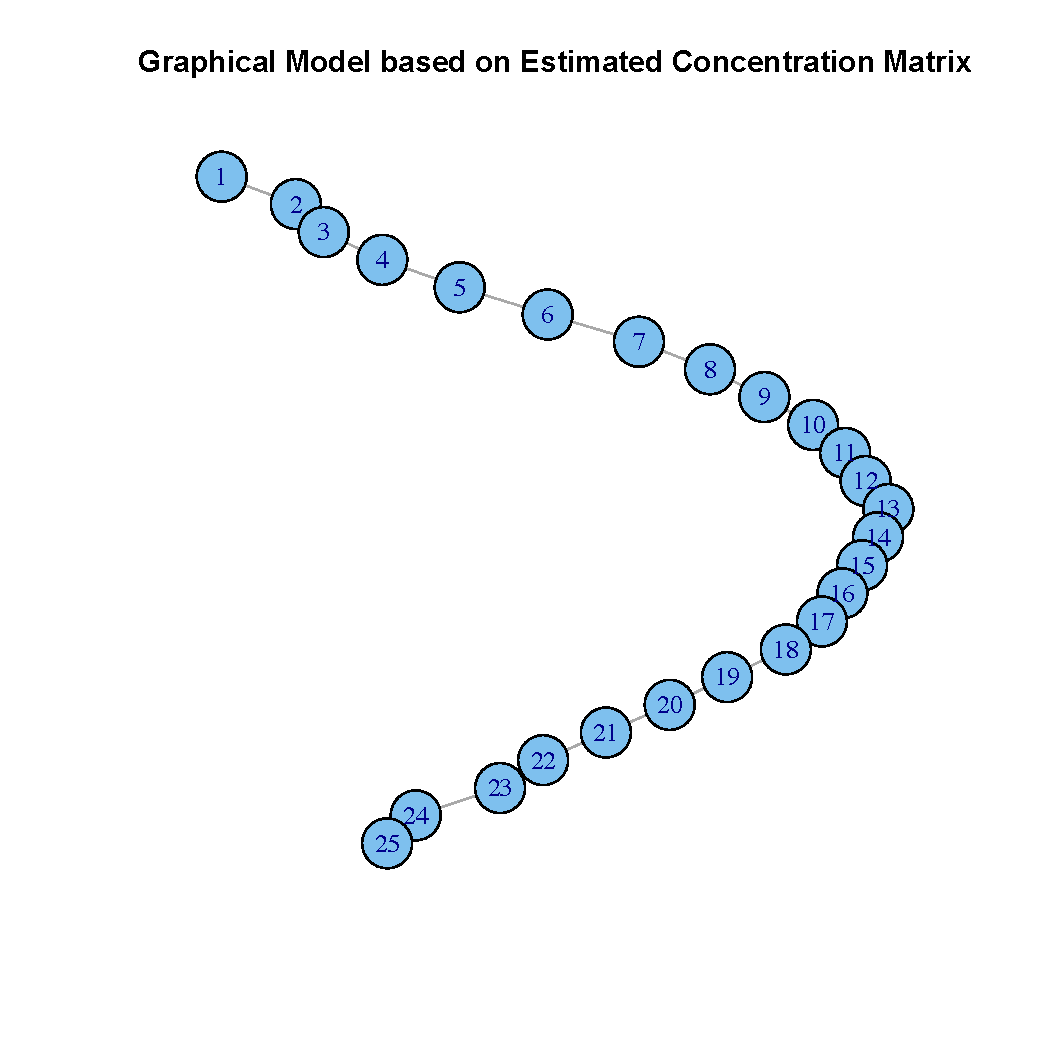
\includegraphics[width=\textwidth]{chaingraphicalmodelestimate.pdf}
  \caption{Estimated Chain Graph}
\label{fig:chaingaphsestimate}
\end{subfigure}\\
\begin{subfigure}[b]{0.5\textwidth}
  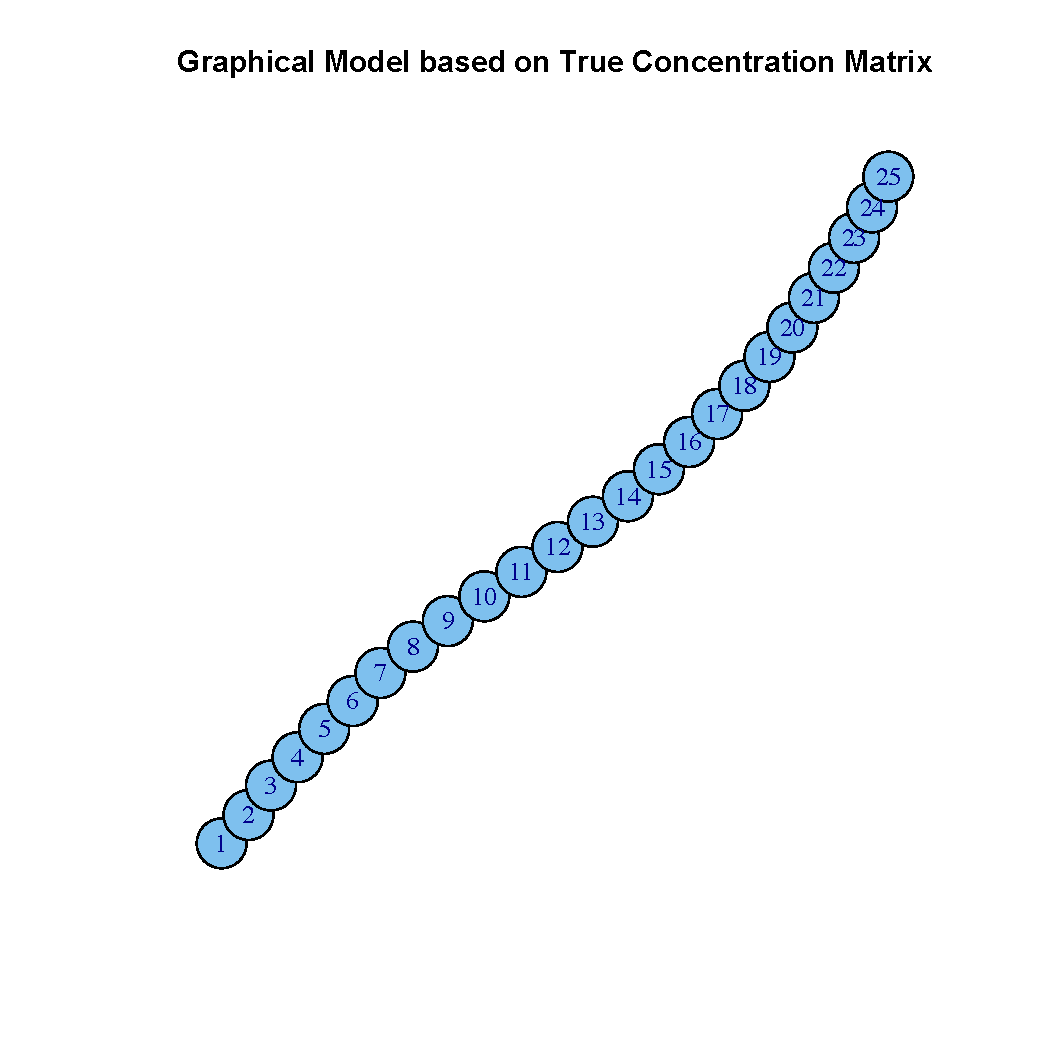
\includegraphics [width=\textwidth]{chaingraphicalmodelactual.pdf}
  \caption{True Chain Graph}
\label{fig:chaingaphsactual}
\end{subfigure}
        \caption{As we can see from the graphs, the sparstiy in the
          case of the chain graphs was predicted exactly.}\label{fig:chaingraphs}
\end{figure}
\begin{figure}
\centering 
\begin{subfigure}[b]{0.5\textwidth}
                \includegraphics[width=\textwidth]{{nearestfpfn.pdf}}
                \caption{False Positive/False Negative rate vs $\lambda$.}
                \label{fig:fpnear}
        \end{subfigure}\\
\begin{subfigure}[b]{0.5\textwidth}
                \includegraphics[width=\textwidth]{{nearestFrobenius.pdf}}
                \caption{Frobenius Norm Loss vs $\lambda$.}
                \label{fig:Frobeniusnear}
        \end{subfigure}
        \caption{Plots for Proximal Gradient Algorithm for Nearest
          Neighbor Graph. $\lambda \approx 15$ seems to be optimal to
          minimize FN/FP while $\lambda \approx 30$ minimizes
          F.}\label{fig:near}
\end{figure}

\begin{figure}
\centering 
\begin{subfigure}[b]{0.40\textwidth}
  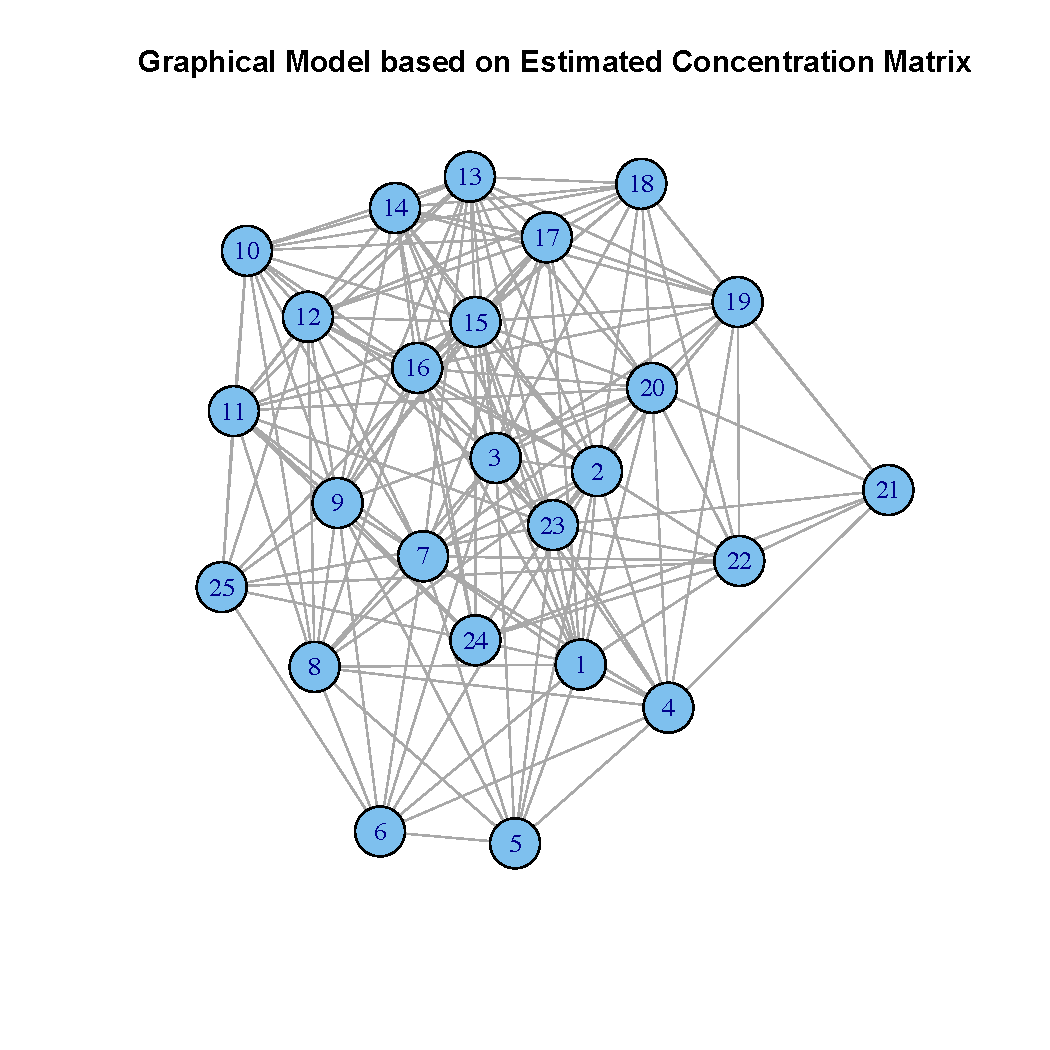
\includegraphics[width=\textwidth]{nearestestimategraph15.pdf}
  \caption{Estimated Nearest Neighbor Graph at $\lambda = 15$}
\label{fig:nearestgaphsestimate}
\end{subfigure}
\begin{subfigure}[b]{0.40\textwidth}
  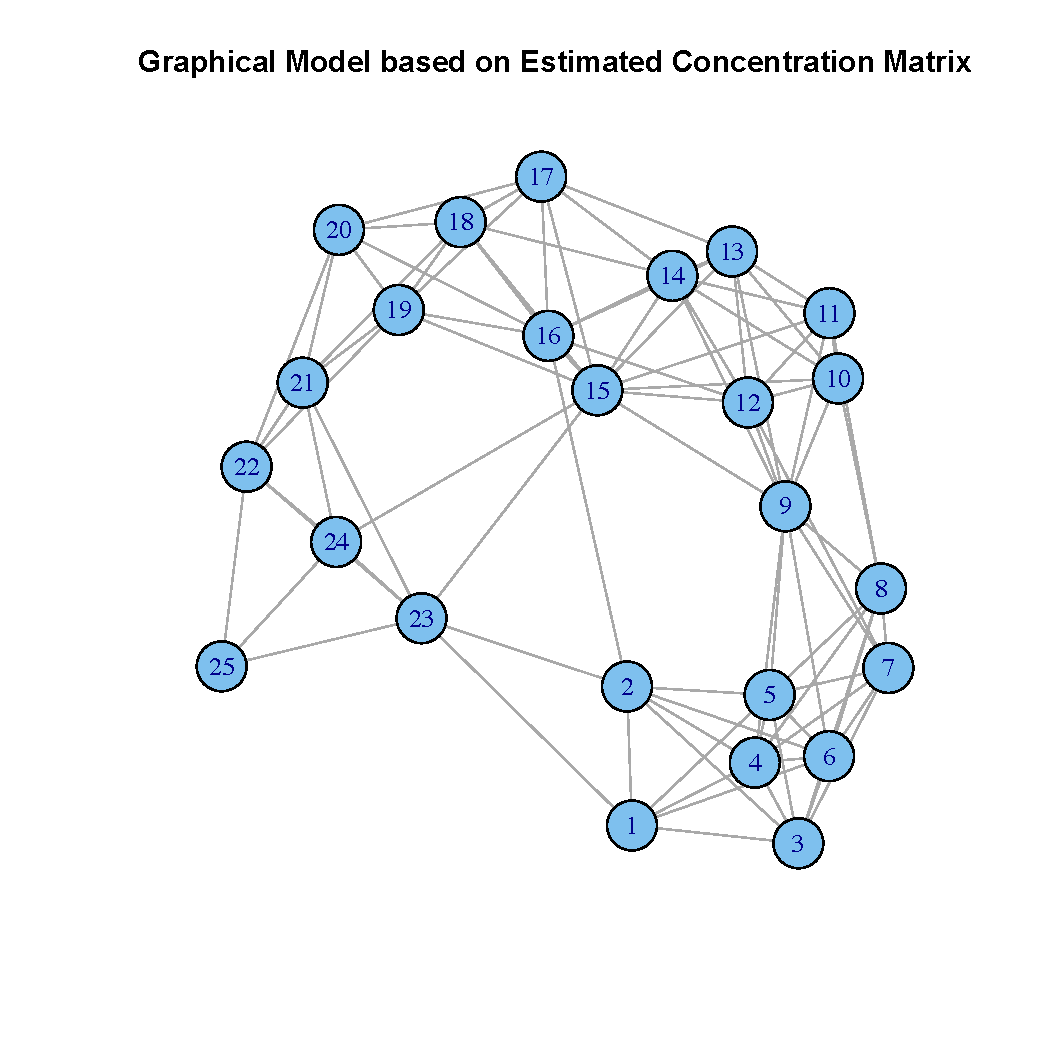
\includegraphics[width=\textwidth]{nearestestimategraph30.pdf}
  \caption{Estimated Nearest Neighbor Graph at $\lambda = 30$}
\label{fig:nearestgaphsestimate}
\end{subfigure}\\
\begin{subfigure}[b]{0.50\textwidth}
  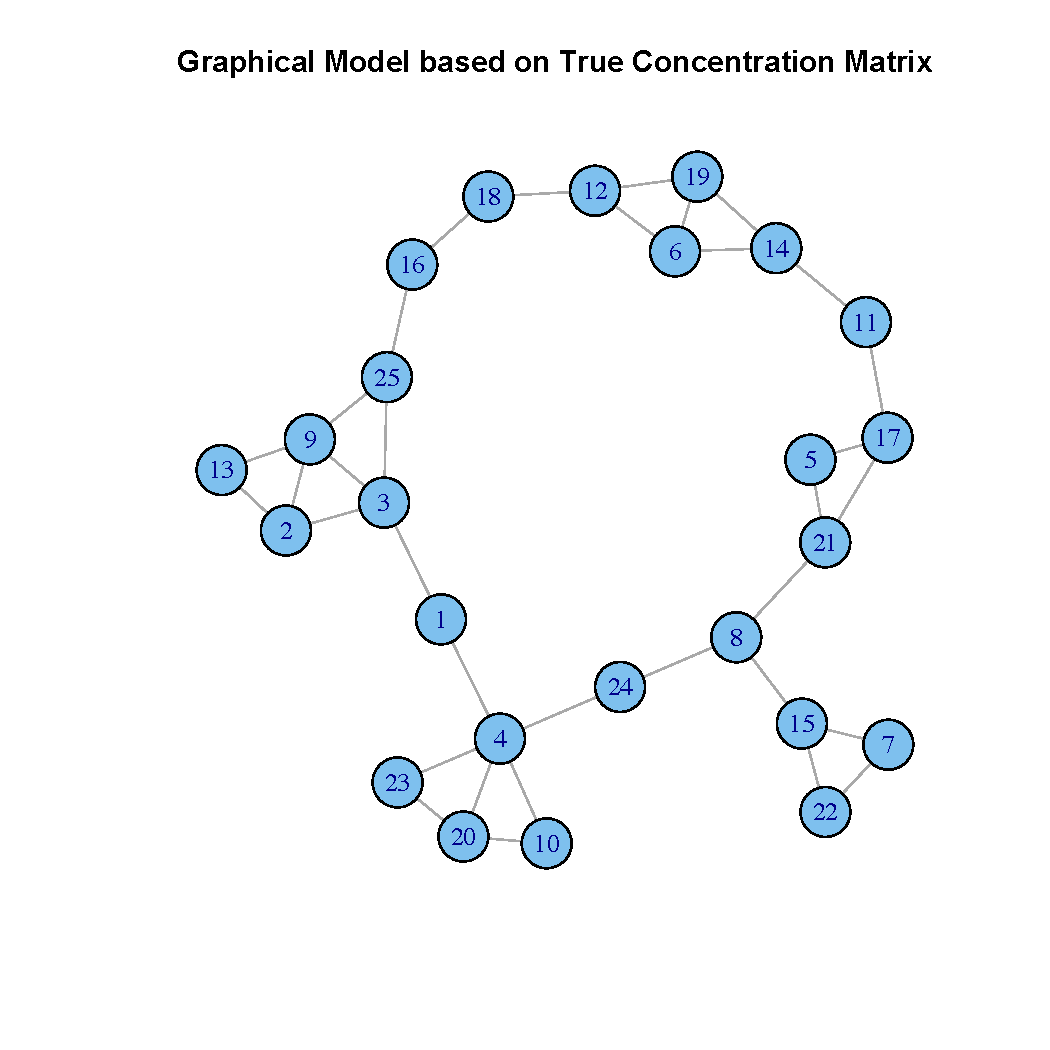
\includegraphics [width=\textwidth]{nearestactualgraph.pdf}
  \caption{True Nearest Neighbor Graph}
\label{fig:nearestgaphsactual}
\end{subfigure}
        \caption{The graph shows the sparsity patterns in the
          estimated and actual graphs in the case of the nearest
          neighbor network. In this case, we were unable to recover
          the exact sparsity pattern.}\label{fig:neargraph}
\end{figure}

\begin{figure}
\centering 
\begin{subfigure}[b]{0.5\textwidth}
                \includegraphics[width=\textwidth]{{barafpfn.pdf}}
                \caption{False Positive/False Negative rate vs $\lambda$.}
                \label{fig:fpbara}
        \end{subfigure}\\
\begin{subfigure}[b]{0.5\textwidth}
                \includegraphics[width=\textwidth]{{baraFrobenius.pdf}}
                \caption{Frobenius Norm Loss vs $\lambda$.}
                \label{fig:Frobeniusbara}
        \end{subfigure}
        \caption{Plots for Proximal Gradient Algorithm for Scale-free
          Network. $\lambda \approx 15$ minimizes FN/FP while $\lambda
          \approx 7$ seems to minimize F .}\label{fig:bara}
\end{figure}

\begin{figure}
\centering 
\begin{subfigure}[b]{0.40\textwidth}
  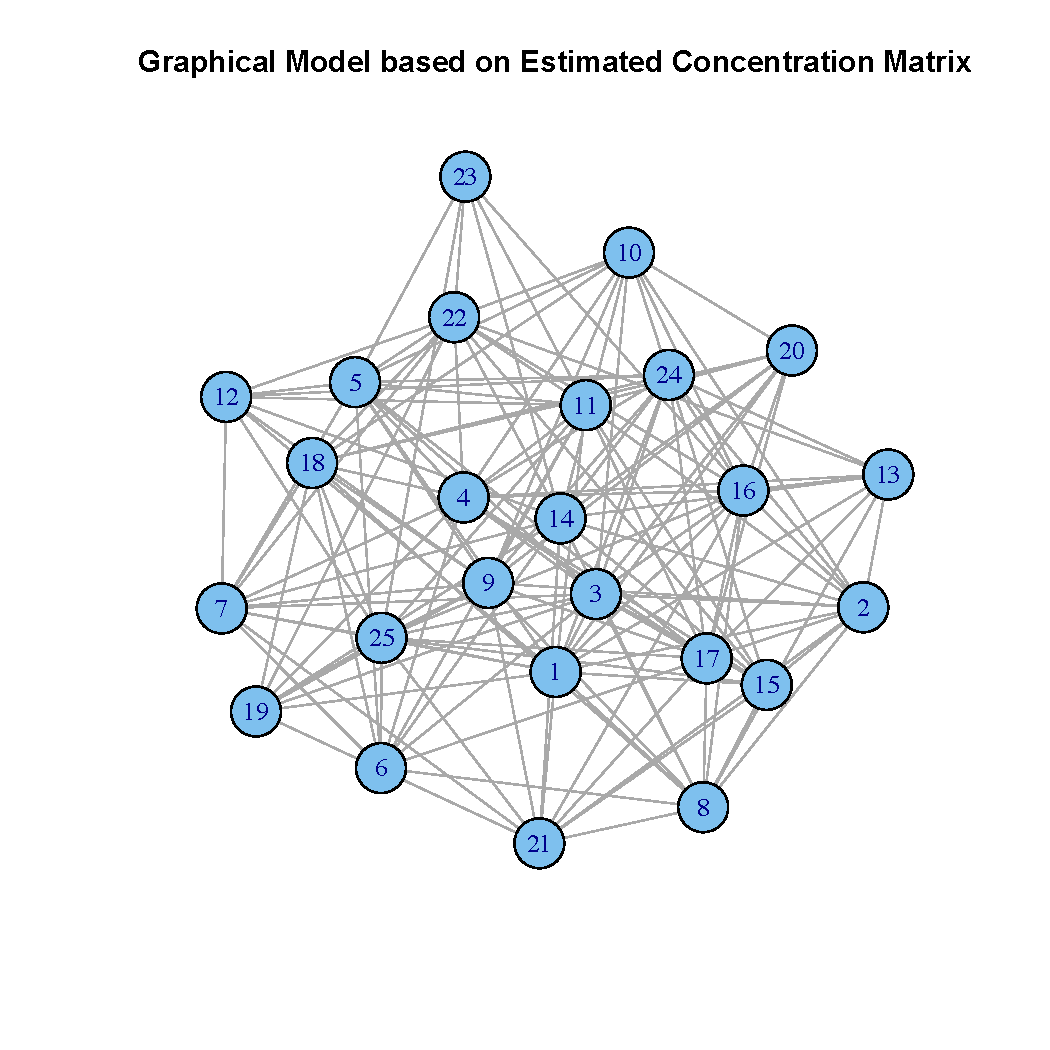
\includegraphics[width=\textwidth]{barabasigraphestimate7.pdf}
  \caption{Estimated Scale-free network Graph at $\lambda = 7$}
\label{fig:nearestgaphsestimate}
\end{subfigure}
\begin{subfigure}[b]{0.40\textwidth}
  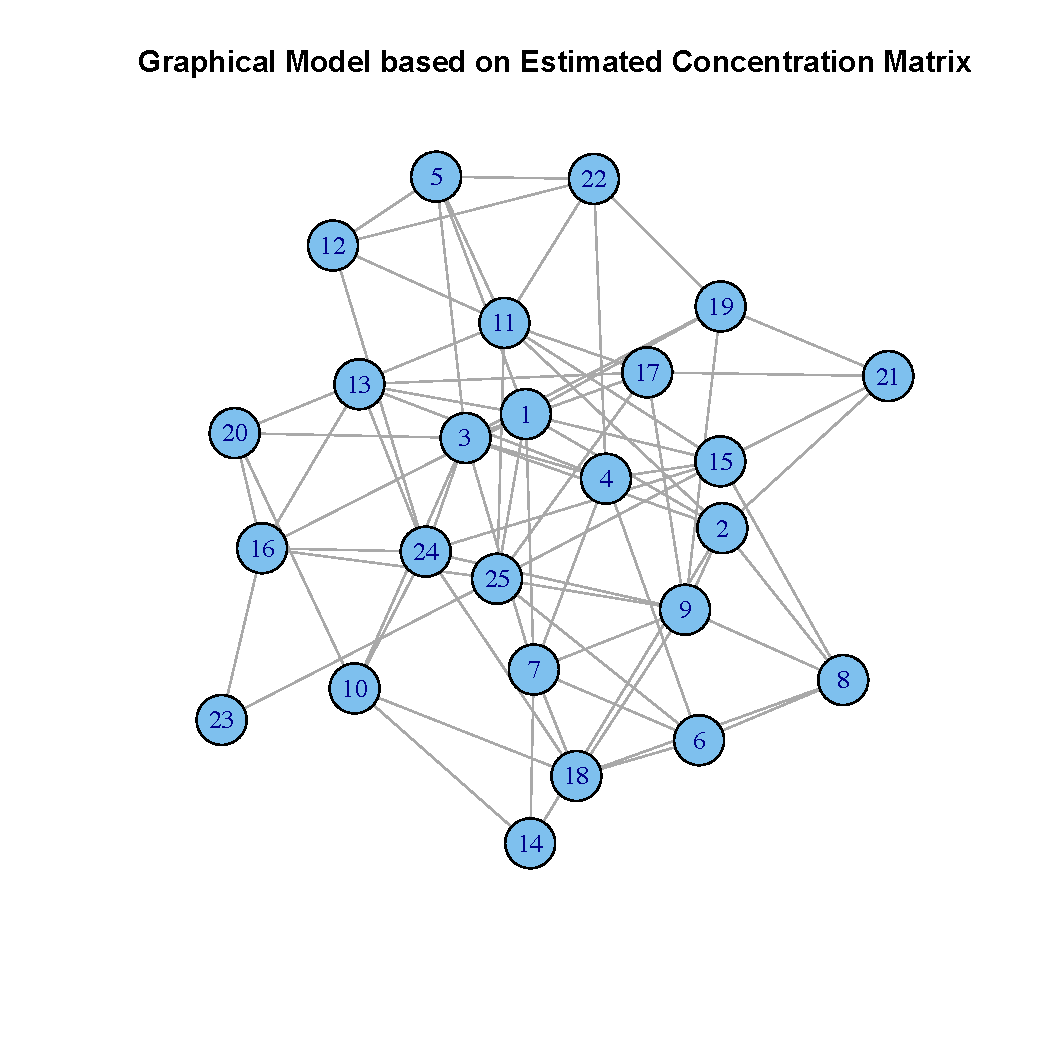
\includegraphics[width=\textwidth]{barabasigraphestimate15.pdf}
  \caption{Estimated Scale-free network Graph at $\lambda = 15$}
\label{fig:nearestgaphsestimate}
\end{subfigure}\\
\begin{subfigure}[b]{0.50\textwidth}
  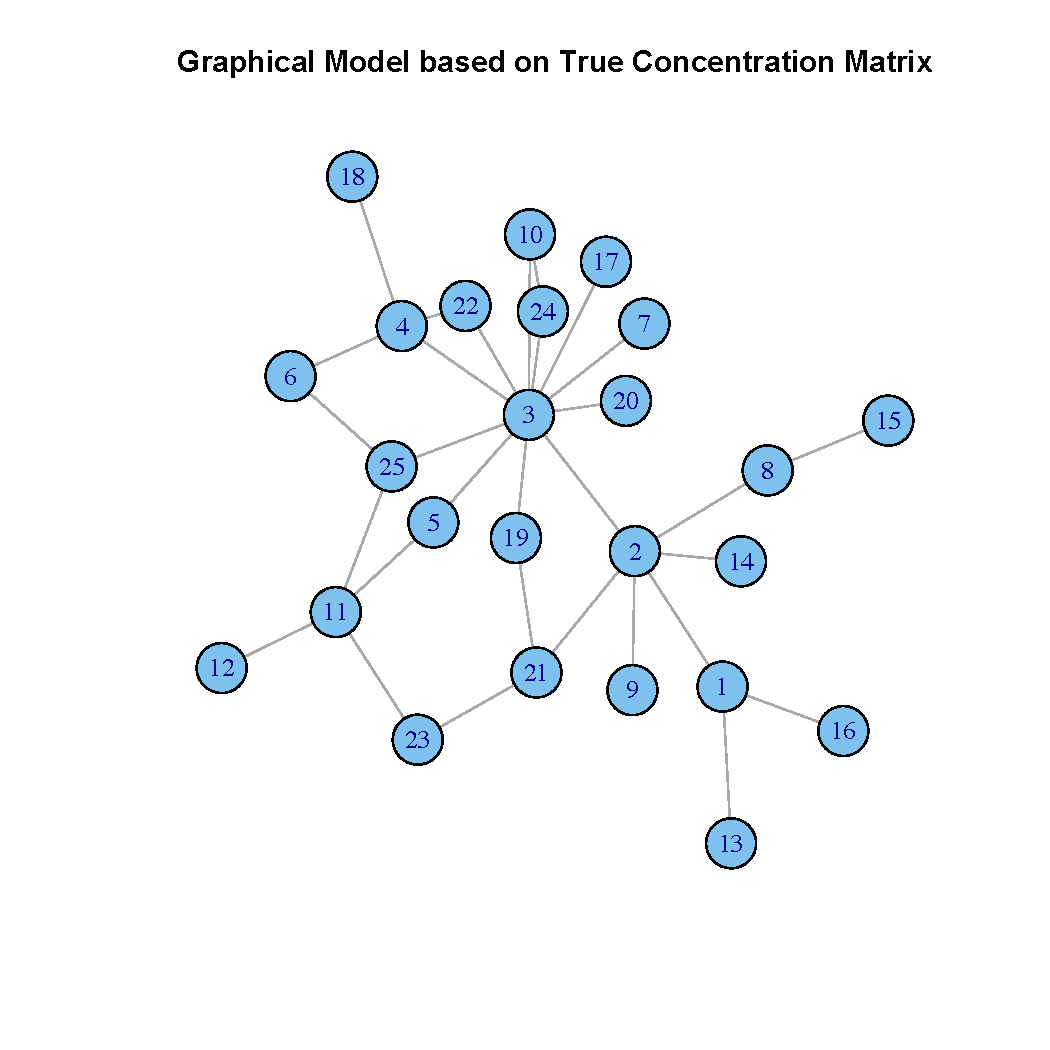
\includegraphics [width=\textwidth]{barabasigraphactual.pdf}
  \caption{True Scale-free network Graph}
\label{fig:nearestgaphsactual}
\end{subfigure}
        \caption{The graph shows the sparsity patterns in the
          estimated and actual graphs in the case of the Scale-free network. In this case also, we were unable to recover
          the exact sparsity pattern.}\label{fig:baragraph}
\end{figure}

\pagebreak 

\paragraph{Appendix: R Code for Proximal Gradient Algorithm}
\begin{verbatim}
                                        #replications
(pdfrobeniusnorm = 0)
(frobeniusnorm = 0)
(fp = 0)
(fn = 0)
for (K in 1:10){
Omega1 = chain(p)
Sigma1 = solve(Omega1)

Y = mvrnorm(n, mu, Sigma1, tol = 1e-6, empirical = FALSE, EISPACK = FALSE)
Y = scale(Y, center = TRUE, scale = TRUE)

(omegahat = diag(p))
(allnodes = seq(1:p))
for(node in 1:p){
    (y = Y[,node])
    (allothernodes = setdiff(allnodes,node))
    (X = Y[,allothernodes])
    (betaold = matrix(0,dim(X)[2],1))
    
    stepsize = 0.0001
    lambda = 60
    iter = 1
    maxIter = 10000
    delta = 10^(-5)
    eps = 1
    while(iter<maxIter && eps>delta){
        (betanew = betaold - stepsize*grad(y,X,betaold,lambda))
        (betanew = softthresh(betanew,stepsize*lambda))
        (eps = norm(betanew - betaold))
        (betaold = betanew)
        (iter = iter + 1)
        ###(stepsize = stepsize/sqrt(iter))  #using diminishing stepsize
        ###(stepsize = stepsize) #using fixed stepsize
    }
    omegahat[node,allothernodes] = betanew
}
(adjmatrixhat = (abs(omegahat)>10^(-5)))
(adjmatrix = (abs(Omega1)>10^(-5)))
pdomegahat = makesymmetric(omegahat)
while(min(eigen(pdomegahat)$value)<0){
    pdomegahat = boostdiagonal(pdomegahat)}
(adjmatrixhat = (abs(pdomegahat)>10^(-5)))
(zero = medgeset(adjmatrixhat))
if(dim(zero)[1]>0){
    (omegahat = glasso(S,0,zero=zero)$wi)}
else{glasso(S,0)$wi}
(adjmatrixhat = (abs(omegahat)>10^(-5)))
(pdfrobeniusnorm[K] = (norm((pdomegahat-Omega1), type = c("F"))^2)
/(norm((Omega1), type = c("F"))^2))
(frobeniusnorm[K] = (norm((omegahat-Omega1), type = c("F"))^2)
/(norm((Omega1), type = c("F"))^2))
(fp[K] = (sum((upper.tri(adjmatrixhat,diag=FALSE)*adjmatrixhat
-upper.tri(adjmatrix,diag=FALSE)*adjmatrix)>0))
/(sum(upper.tri(adjmatrix,diag=FALSE)*adjmatrix==0)-(1/2)*(p)*(p+1)))
(fn[K] = (sum(upper.tri(adjmatrix,diag=FALSE)*adjmatrix-
upper.tri(adjmatrixhat,diag=FALSE)*adjmatrixhat>0))
/(sum(upper.tri(adjmatrix,diag=FALSE)*adjmatrix>0)))     
}
\end{verbatim}

\end{document}